\documentclass{report}
\usepackage{pgfplots, color}

\begin{document}

  \title{Test sur LaTeX et les graphes}
  \author{Alexis Opolka\ 26B Avenue Charles de Gaulle}
  \date{\today}
  \maketitle

  \begin{abstract}
    C'est un document relatant d'expérimentations sur le langage LaTeX et
    le moteur TeX afin de pouvoir développer une extension permettant d'intégrer
    du langage LaTeX à du Markdown.

    Ceci comprend des graphes, des notes de bas de page, etc.
  \end{abstract}

  \tableofcontents
  \listfigurename

  \newpage

  \[
    \lim_{x\to0} \frac{\cos{(2x)} - 1}{x^3 + 5x^3}
  \]

  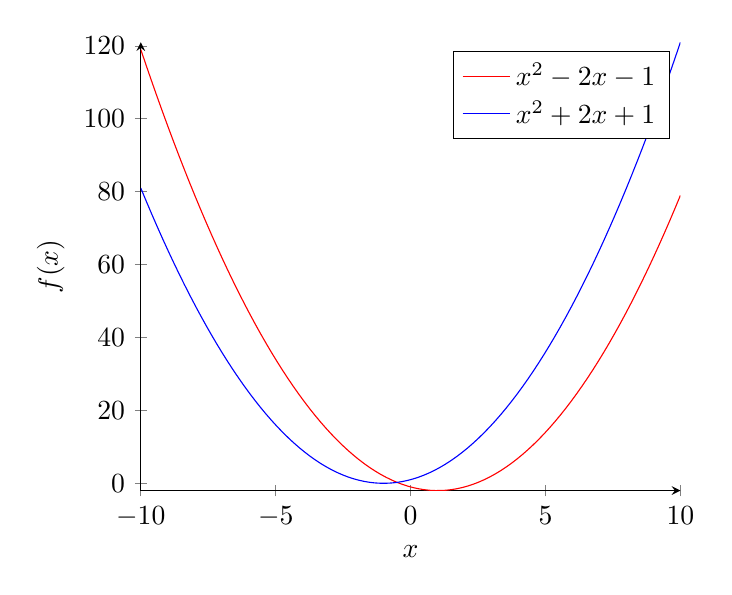
\begin{tikzpicture}
    \begin{axis}[
      axis lines = left,
      xlabel = \(x\),
      ylabel = {\(f(x)\)},
    ]
    % The red parabola is defined
    \addplot[
      domain = -10:10,
      samples = 100,
      color = red,
    ] {x^2 - 2*x - 1};
    \addlegendentry{\(x^2 - 2x - 1\)}
    % The blue parabola is defined
    \addplot [
      domain = -10:10,
      samples = 100,
      color = blue,
    ] {x^2 + 2*x + 1};
    \addlegendentry{\(x^2 + 2x + 1\)}
    \end{axis}
  \end{tikzpicture}

  \end{document}
